\documentclass[12pt]{article}

\usepackage{sbc-template}

\usepackage{graphicx,url}

\usepackage[brazil]{babel}   
%\usepackage[latin1]{inputenc}  
\usepackage[utf8]{inputenc}  
% UTF-8 encoding is recommended by ShareLaTex

\usepackage{subfigure}
\usepackage{multirow}

\usepackage{verbatim}

\usepackage{amssymb,amsfonts,amsmath}

\usepackage{xcolor}
% Definindo novas cores
\definecolor{verde}{rgb}{0,0.5,0}
% Configurando layout para mostrar codigos C++
\usepackage{listings}
\lstset{
  language=C++,
  basicstyle=\ttfamily\small, 
  keywordstyle=\color{red}, 
  stringstyle=\color{blue}, 
  commentstyle=\color{gray}, 
  extendedchars=false, 
  showspaces=false, 
  showstringspaces=false, 
  numbers=left,
  numberstyle=\tiny,
  breaklines=true, 
  backgroundcolor=\color{white!10},
  breakautoindent=true,
  captionpos=b,
  xleftmargin=0pt,
}

\sloppy

\title{Relatório de Avaliação de Rede Sem Fio IEEE 802.11 em modo Infraestruturado no simulador \textit{Network Simulator 3}}

\author{Joahannes B. D. da Costa\inst{1}, Wellington V. Lobato Junior\inst{1}}

\address{Laboratório de Redes de Computadores (LRC) -- Instituto de Computação (IC)\\
Universidade Estadual de Campinas (UNICAMP)\\
  Campinas -- São Paulo -- Brasil
  \email{\{joahannes,wellington\}@lrc.ic.unicamp.br}
}

\begin{document} 

\maketitle

\begin{resumo} 
Este documento apresenta uma avaliação da comunicação de rede sem fio 802.11 em modo infraestruturada e é parte dos critérios de avaliação da disciplina MO655 - Gerência de Redes de Computadores, do Instituto de Computação (IC), da UNICAMP, sob supervisão do Prof. Dr. Edmundo Madeira. Desta forma, os tráfegos de comunicação gerados foram o de Constant Bit Rate (CBR), utilizando o protocolo UDP, e tráfego em Rajadas, que por sua vez utiliza o protocolo TCP. O número de clientes conectados na rede varia de 1 a 6. Ainda, dois cenários de mobilidade foram utilizados, o primeiro sendo os nós parados em volta do AP e o segundo com os clientes se deslocando até a borda da rede. Os resultados mostraram que a presença de mobilidade nos nós influencia diretamente nas taxas de atraso, vazão e perda de pacotes. 
\end{resumo}


\section{Introdução}

%512kbps/8 = Bs/512 bytes = pacotes/s por 60 = pacote

O surgimento de várias tecnologias nos últimos anos é decorrência do avanço nas tecnologias de comunicação, que procuram sempre atendar as necessidades e demandas de seus usuários com a melhor qualidade possível. Especialmente a comunicação sem fio ganhou espaço considerável no universo de transmissão de dados, deixando de existir apenas nas comunicações de longa distância, como em satélites, para fazer parte de ambientes locais. Essa utilização mais comum foi fortalecida pelo investimento da academia e indústria no sentido de aplicar a comunicação sem fio em redes de computadores \cite{gtaredesemfio}.

Os primeiros produtos para redes sem fio começaram a sere introduzidos no início da década de 90. Dentro deste contexto notou-se que faltava uma padronização de uso e compatibilidade, observando esta lacuna o IEEE (\textit{Institute of Electrical and Eletronics Engineers}) desenvolveu e aprovou normas para o uso, ficando conhecidas como IEEE 802.11, tendo sua primeira versão publicada em 1997 \cite{batalha2018}. O padrão 802.11 não parou na primeira versão Experimental \cite{tanenbaum2003computer}, ao decorrer dos anos a tecnologia sofreu evoluções e com elas novas opções para o seu uso e manuseio.

O padrão IEEE 802.11 define basicamente uma arquitetura para as Redes Locais Sem Fio (\textit{Wireless Local Area Network - WLAN}) que abrange os níveis físico e de enlace. Transmissões com frequência de rádio são consideradas no nível físico, embora outras formas de transmissão sem fio possam ser usadas, como microondas, infravermelho e laser. Para o nível de enlace, o IEEE definiu um protocolo de controle de acesso ao meio (protocolo MAC), bastante semelhante ao protocolo usado em redes locais Ethernet (CSMA/CD) \cite{gtaredesemfio}. O padrão IEEE 802.11 possibilita a transmissão de dados numa velocidade que atingem até 1300 Mbit/s (IEEE 802.11ac) \cite{cisco80211ac, bejarano2013ieee}.

Levando isso em consideração, este documento traz algumas avaliações realizadas em uma Rede Sem Fio 802.11 em modo infraestruturado. São utilizados 3 tipos de tráfegos diferentes, sendo CBR, Rajada e CBR/Rajada. Ainda, os impactos da adição de mobilidade aos clientes conectados à rede também são analisados.

O restante deste relatório está organizado como se segue. A Seção \ref{fundamentacao} apresenta uma revisão da literatura de conceitos utilizados neste experimento. Na Seção \ref{avaliacao} as características do exercício proposto, o software utilizado nas simulações e definições importantes para o entendimento do trabalho.  A Seção \ref{resultados} apresenta os resultados obtidos nos experimentos. Finalmente, a Seção \ref{consideracoes} apresenta as considerações finais acerca dos resultados e do experimento como um todo. \textbf{Vale ressaltar que ao final deste documento encontram-se os principais códigos utilizados nas simulações}.

\section{Fundamentação Teórica}
\label{fundamentacao} 
Esta Seção descreve os conceitos de redes de computadores utilizados para realizar as simulações. Aqui são descritos os protocolos utilizados, bem como os conceitos relacionados as métricas coletadas.

\subsection{Protocolo UDP}

O protocolo UDP (\textit{User Datagram Protocol}) é um protocolo não orientado à conexão da camada de transporte do modelo TCP/IP. Ele não fornece nenhum tipo de tratamento e controle de erros por isso é considerado como um protocolo simples. De forma resumida, o UDP recebe mensagens do processo da aplicação que deseja enviar dados, anexa os campos de número de porta de origem e destino para o serviço de multiplexação/demultiplexação e transmite o segmento resultante para a camada de rede. A camada de rede encapsula o segmento da camada de transporte em um datagrama\footnote{O datagrama IP é a unidade básica de dados no nível IP} IP e, em seguida, faz uma tentativa de melhor esforço para entregar o segmento ao destinatário \cite{kurose2013computer}.

Se o segmento conseguir chegar ao destinatário, o UDP usará o número da porta de destino para entregar os dados do segmento ao processo da aplicação correto. Observe que, com o UDP, não há \textit{handshaking} entre o envio e o recebimento de entidades da camada de transporte. Por essa razão, o UDP é dito como não orientado à conexão. O objetivo dele é acelerar o processo de envio de dados, visto que todas as etapas de comunicação necessárias para verificar a integridade de um pacote contribuem para deixá-lo mais lento.

Ou seja, quando o protocolo UDP é acionado, ele apenas manda informações a um destinatário, sem a preocupação se elas irão ser recebidas de forma correta. Caso ocorram erros, simplesmente envia o próximo pacote e os anteriores não podem ser recuperados. Esse método garante uma comunicação rápida entre dois computadores, mesmo potencializando a ocorrência de erros. Graças à essas características, o protocolo é bastante usado em situações nas quais a correção de erros não é exatamente desejada, como \textit{streamings} de vídeo ou jogos \textit{online}, por exemplo. 

%Durante a transmissão de um vídeo ao vivo, por exemplo, é mais interessante que uma pessoa perca alguns trechos ou tenha que lidar com distorções de imagem e áudio do que esperar pelo recebimento de um pacote que se perdeu - o que pode acabar com o fator ``tempo real".

\subsection{Protocolo TCP}

O Protocolo de Controle de Transmissão, ou apenas TCP (\textit{Transmission Control Protocol}) é um dos principais protocolos da camada de transporte do modelo TCP/IP e é conhecido por ser o protocolo de transporte da Internet, confiável e orientado à conexão \cite{kurose2013computer}. Ele permite gerenciar os dados vindo da camada inferior do modelo (ou seja, o protocolo IP). Quando os dados são fornecidos ao protocolo IP, este encapsula-os em datagramas IP. O TCP é um protocolo orientado à conexão, ou seja, ele permite que duas máquinas se comuniquem entre elas durante o processo de envio, que é conhecido como \textit{handshaking}, além de controlar o estado da transmissão.

O TCP não só envia os dados como também recebe informações para se assegurar que os pacotes foram recebidos sem erros. Ele também adota um mecanismo próprio para se assegurar que os pacotes enviados vão chegar ao destino na ordem correta. Caso o receptor não receba um pacote corretamente, a informação é enviada novamente até que chegue de forma correta ao destino. Também há uma checagem se as informações não foram corrompidas no trajeto entre emissor e receptor.

% É exatamente essa a característica que se destaca no protocolo: a confiabilidade. É graças ao TCP que os downloads que você faz não são corrompidos por oscilações na velocidade de sua conexão e que as páginas acessadas por seu navegador dificilmente deixam de carregar algum elemento por acidente — é claro, se uma das máquinas usadas para a troca de dados ficar offline durante esse processo, você receberá uma mensagem de erro e não conseguirá acessar o conteúdo que deseja.

\subsection{Definições}

\begin{itemize}
    \item \textbf{Intervalo de confiança}: Um intervalo de confiança (IC) é um intervalo estimado de um parâmetro de interesse de uma população. Em vez de estimar o parâmetro por um único valor, é dado um intervalo de estimativas prováveis. Intervalos de confiança são usados para indicar a confiabilidade de uma estimativa \cite{shimakura2012}.
    \item \textbf{Vazão}: A vazão é definida como o número de bits que podem ser transmitidos sobre a rede num dado tempo, sendo expressa em bits/segundo (b/s). Por exemplo, numa rede Ethernet podemos ter como vazão 10Mb/s. Muitas vezes usa-se o termo taxa de transmissão para se referir a vazão \cite{ifprvazao}.
    \item \textbf{Atraso}: O atraso é o tempo que um pacote leva para atravessar uma rede desde a origem até o destino, passando pelos roteadores e enlaces intermediários. Ao percorrer uma rede, um pacote sofre uma série de atrasos em cada um dos nós do caminho. Este atraso em cada nó da rede tem quatro componentes principais: o atraso de processamento, o atraso de fila, o atraso de transmissão e o atraso de propagação \cite{ifprvazao}.
    \item \textbf{Perda de pacotes}: A perda de pacotes ocorre quando a capacidade de armazenamento da fila de um roteador se esgota. Neste caso os novos pacotes que chegam são descartados (\textit{dropped}) e são considerados perdidos. A fração dos pacotes perdidos aumenta a medida que a intensidade de tráfego aumenta. Pacotes corrompidos totalmente também podem ser considerados como perdidos \cite{ifprvazao}.
    \item \textbf{Tráfego CBR}: Aplicado a conexões que necessitam de banda fixa (estática) devido aos requisitos de tempo bastante apertados entre a origem e o destino. Aplicações típicas deste serviço são: áudio interativo (telefonia), distribuição de áudio e vídeo (televisão, pay-per-view, etc), e áudio e vídeo \textit{on demand} \cite{em2012disponivel}.
    \item \textbf{Tráfego em Rajada}: Aplicado a conexões que transportam tráfego em rajadas que necessitam de garantia de banda, embora a taxa de bits possa variar. Aplicações típicas deste serviço são as interligações entre redes e a emulação de LAN’s \cite{em2012disponivel}.
\end{itemize}

\section{Exercício proposto}
\label{exercicio}

O exercício proposto para as avaliação se refere à simular uma Rede sem Fio 802.11 no modo infraestruturado com um Ponto de Acesso (\textit{Access Point - AP}). Mostrar Vazão, Atraso e Perda de Pacotes para um dispositivo móvel que se move do \textit{AP} para a borda da rede. Em seguida, mostrar Vazão, Atraso e Perda  para os casos de $2$, $4$ e $6$ dispositivos móveis transmitindo simultaneamente, nos cenários com e sem mobilidade. Considerar a Rede sem Fio conectada à Internet por um enlace cabeado de $100$ Mbps.

Usar tráfego em rajadas e fontes CBR (\textit{Constant Bit Rate}). Tamanho de quadro: 512 (CBR) e 1500 bytes (Rajada). Mostrar os resultados para tráfego TCP, UDP e 50\% de cada, chamada aqui de CBR/Rajadas, (usar intervalo de confiança de 95\%).

\section{Avaliação}
\label{avaliacao}

Esta seção descreve a metodologia e métricas utilizadas para avaliar a eficiência das aplicações de CBR, Rajada e CBR/Rajada em termos de atraso médio, vazão e número pacotes perdidos. Foram realizadas simulações com diferentes números de clientes a fim de identificar o impacto disso para a rede.

\subsection{Metodologia}
\label{subsec:metodologia}

As simulações foram realizadas no Network Simulator 3 (NS3)\footnote{\url{https://www.nsnam.org/}}, o qual implementa a pilha de protocolo do padrão IEEE 802.11a para comunicação e atenuação de sinal. O IEEE 802.11a está definido como padrão no NS3 por isso optou-se por utilizá-lo neste trabalho. Para estabelecer um cenário de avaliação, utilizou-se uma área de $140$m x $140$m. Para os nós estáticos foi utilizado o modelo de mobilidade \texttt{ConstantPositionMobility} e para o cenário com mobilidade foi utilizado o modelo \texttt{ConstantVelocityMobility}, ambos fornecido pelo NS3.

A taxa de dados foi definida em $512$ kbits e a potência de transmissão em $16$ dbm, conforme padrão estabelecido no modelo \texttt{YansWifiPhy} do NS3\footnote{\url{https://www.nsnam.org/doxygen/classns3_1_1_yans_wifi_phy.html}}. Esses parâmetros, juntamente com o modelo de propagação \texttt{FriisPropagationLossModel}, fornecem um raio de comunicação de $\sim70$ metros. Cada simulação foi executada $33$ vezes com diferentes sementes de aleatoriedade e os resultados apresentam os valores com um intervalo de confiança de $95$\%. O tempo de simulação foi de $60$ segundos.

Para quantificar a evolução do tráfego neste cenário, variou-se o número de clientes conectados à rede em $1, 2, 4$ e $6$ dispositivos. Ainda, dois cenários de mobilidade foram definidos. O primeiro com ausência de mobilidade, onde os nós são dispostos próximos ao AP e ficam estáticos até o final da simulação. No segundo cenário, os nós clientes possuem mobilidade que varia entre $1$ e $2$ m/s (igual a $3.6$ e $7.2$ km/h), o que se aproxima da mobilidade de pessoas caminhando. Considerou-se que os clientes se distanciam do AP até próximo à borda da rede.

A conexão estabelecida entre o \textit{Router}, que representa a Internet, e o \textit{AP} se dá através de um enlace Ethernet de 100Mbps com atraso de 2 milissegundos, conforme especificação padrão do próprio NS3 através da classe \texttt{ns3::CsmaHelper}. O algoritmo utilizado para controle de taxa foi o AARF que é disponibilizado através da classe \texttt{ns3::AarfWifiManager}. Controle de taxa é a determinação da taxa de transmissão de dados ideal mais apropriada para as condições atuais do canal sem fio. Consiste em avaliar as condições do canal e, consequentemente, ajustar a taxa. A adaptação da taxa é bastante desafiadora devido às flutuações das condições do canal \cite{lacage2004ieee, wong2006robust}.

A organização dos dispositivos no cenário se dá da seguinte forma: o $Router$ está posicionado nas coordenadas $x=0,y=0$, o \textit{AP} está posicionado no centro do cenário ($x = 70, y = 70$), e os clientes são alocados em suas posições iniciando de $x=70,y=70$ com $\Delta X = 5$, $\Delta Y = 5$ e organização de layout $RowFirst = 3$. Tais configurações fazem que o primeiro cliente fique bem embaixo do \textit{AP}, cada cliente fique à 5 metros de distância um do outro e organizados em grupos de 3 em 3 por linha, conforme ilustrado na Figura \ref{fig:cenario}.

\begin{figure}[ht]
	\centering
	\includegraphics[width=0.65\textwidth]{img/cenario_mo655.png}
	\caption{Cenário dos experimentos.}
	\label{fig:cenario}
\end{figure}

Para capturar os resultados gerados em cada simulação foi utilizada a classe de rastreamento de fluxos \texttt{ns3::FlowMonitor}. Ao final de cada simulação, as informações foram guardadas em arquivos de texto e depois tratadas com a linguagem Python para organização e plotagem dos gráficos. Um exemplo do arquivo gerado com 1 cliente e tráfego CBR é exibido abaixo.

\begin{verbatim}
Build commands will be stored in build/compile_commands.json
'build' finished successfully (3.827s)
FlowID[1]   Trafego   CBR
FlowID[1]   Cliente   1
FlowID[1]   Fluxo   10.1.2.2 -----> 192.168.0.2
FlowID[1]   Duracao   58.9903
FlowID[1]   Vazao(Mbps)   0.51693
FlowID[1]   Atraso   0.00215035
FlowID[1]   PacotesTransmitidos   7899
FlowID[1]   PacotesPerdidos   0
\end{verbatim}

A atribuição de tráfego em cada nó cliente é estabelecida através de uma variável chamada $trafego$ que por padrão recebe valor $0$. Assim, quando $trafego = 0$, o tráfego CBR é instalado em todos os clientes e quando $trafego = 1$, o tráfego Rajada é instalado em todos os clientes. Porém, quando o tráfego escolhido for $trafego = 2$, 50\% dos clientes devem utilizar tráfego CBR e os outros 50\% utilizar tráfego em Rajada. Para essa atribuição, é feita uma verificação através do $id$ de cada cliente, conforme mostrado na Equação \ref{eq:trafego}.

\begin{equation}
\label{eq:trafego}
trafego(id) =
	\begin{cases} 
      CBR, &  \text{se } trafego = 0\\
      Rajada, &  \text{se } trafego = 1\\
      CBR/Rajada, & \text{se } trafego = 2  
      ~\begin{cases} 
        CBR, &  \text{se } id \bmod 2 = 0\\
        Rajada, & \text{\textit{Caso contrário}}\\
	  \end{cases}
      \\
	\end{cases}
\end{equation}

% \begin{equation}
% \label{eq:trafego}
% trafego(id) =
% 	\begin{cases} 
%       CBR &  \text{se } $id \% 2 = 0$\\
%       Rajada & \text{Caso contrário}\\
% 	\end{cases}
% \end{equation}

Se um cenário de $trafego = 2$ possuir apenas 1 cliente, o mesmo receberá o tráfego CBR, já que o $id$ do cliente na estrutura que comporta os nós no simulador (\texttt{NodeContainer}) é igual a $0$ e $0 \bmod 2 = 0$. Porém, se um cenário de mesmo tráfego possuir 2 clientes, o cliente de $id = 0$ receberá o tráfego CBR e o de $id = 1$ receberá o tráfego Rajada, já que $1 \bmod 2 \neq 0$. Tornando assim a simulação com 50\% de tráfego CBR e 50\% de Rajada.

Por fim, a Tabela \ref{tab:parametros_16} resume os parâmetros utilizados nas simulações para ambos os cenários estabelecidos.

\begin{table}[!ht]
\centering
\caption{Parâmetros de simulação para os cenários}
\vspace{0.1cm} %espaco entre titulo e tabela
\label{tab:parametros_16}
\begin{tabular}{ll}
\hline
 \textbf{Parâmetro} & \textbf{Valor} \\
\hline
 Tempo de simulação & 60 s \\
 Número de cliente & 1, 2, 4 e 6 \\
 Tamanho do cenário & 140m x 140m \\
 Padrão de comunicação & IEEE 802.11a \\
 Potência de transmissão & 16 dbm\\
 Velocidade dos clientes no cenário estático & 0 km/h \\
 Velocidade dos clientes no cenário móvel & 3.6 a 7.2 km/h \\
 Modelo de mobilidade para nós estáticos & \texttt{ConstantPositionMobility} \\
 Modelo de mobilidade para nós móveis & \texttt{ConstantVelocityMobility} \\
 Taxa de dados & 512 kbps \\
 Tamanho do quadro UDP & 512 bytes\\
 Tamanho do quadro TCP & 1500 bytes \\
 Número de antenas no AP & 1 \\
 Aplicações & CBR, Rajada e CBR/Rajada\\
\hline
\end{tabular}
\end{table}

\section{Resultados}
\label{resultados}

Os resultados obtidos nas simulações são apresentados nas subseções \ref{subsec:atraso_16}, \ref{subsec:vazao_16} e \ref{subsec:perda_16} referentes ao Atraso, Vazão e Perda de Pacotes, respectivamente. Todos os resultados contam com os 3 tipos de tráfegos utilizados, sendo CBR, Rajada e CBR/Rajada.

\subsection{Atraso}
\label{subsec:atraso_16}

A Figura \ref{fig:atraso} exibe os resultados de atraso, em milissegundos, obtidos nos cenários sem e com mobilidade. Especificamente na Figura \ref{fig:atraso_estatico_16}, pode-se notar que com 1 e 2 clientes conectados o atraso é bem baixo para ambos os tráfegos. No entanto, tem um crescimento com 4 clientes e decaimento com 6 clientes conectados. Especialmente os dispositivos com tráfego CBR tiveram maiores taxas de atraso, seguidos pelo CBR/Rajada e Rajadas. O aumento do atraso do CBR pode ser justificado pelo fato da fila de pacotes do UDP estar enchendo, o que ocasiona aumento no atraso de espera de cada pacote até sua transmissão.

Outro ponto importante é que o aumento do atraso de 2 para 4 clientes conectados ocasionado pelo enchimento da fila de transmissão tem impacto direto no número de pacotes perdidos, já que a fila sem espaço livre faz com que os pacotes que chegam para transmissão sejam perdidos. Esse comportamento será melhor visualizado na Figura \ref{fig:perda_estatico_16} mais à frente.

O gráfico ilustrado na Figura \ref{fig:atraso_mobilidade_16} segue o padrão descrito anteriormente. Porém, podemos notar que a mobilidade presente nos nós faz com que o atraso com 4 e 6 clientes na rede seja maior que o cenário sem mobilidade. Ou seja, a mobilidade faz com que os algoritmos de controle levem em consideração essa movimentação para entrega dos pacotes.

\begin{figure}[ht]
	\centering
	\subfigure[Sem mobilidade]{
	    \includegraphics[width=0.48\textwidth]{img/delay_estatico_1_6.eps}
	    \label{fig:atraso_estatico_16}
	}
	\subfigure[Com mobilidade]{
		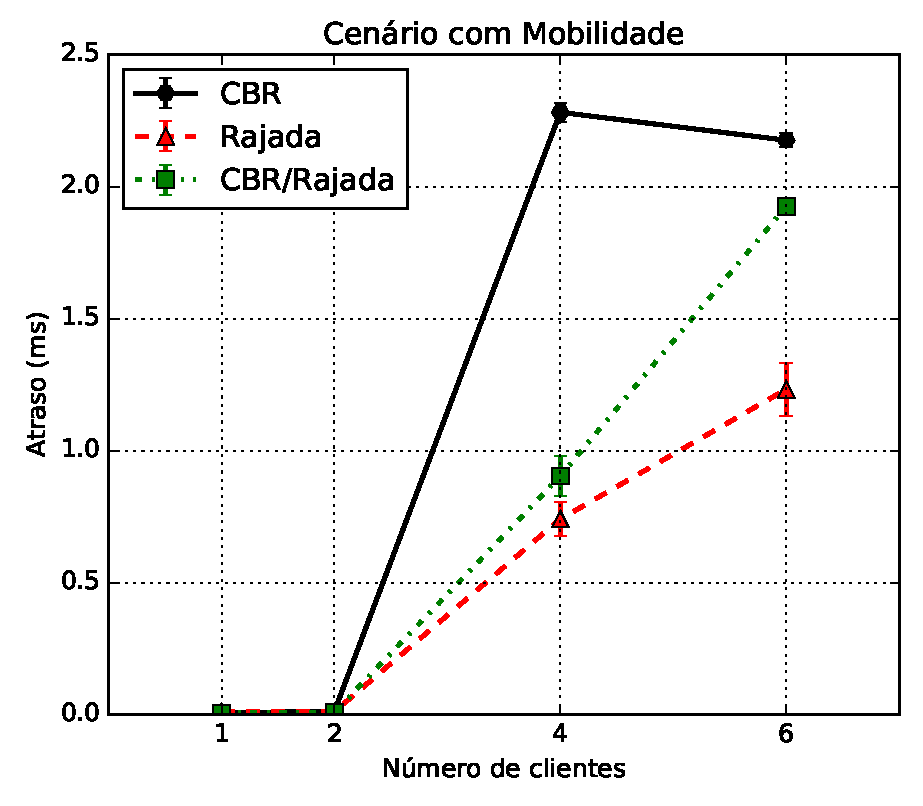
\includegraphics[width=0.48\textwidth]{img/delay_mobilidade_1_6.eps}
	    \label{fig:atraso_mobilidade_16}
	}
	\caption{Resultados de atraso nos cenários sem e com mobilidade.}
	\label{fig:atraso}
\end{figure}

\subsection{Vazão}
\label{subsec:vazao_16}

A Figura \ref{fig:vazao} exibe o resultado de Vazão, em Megabit por segundo (Mbps), nos cenários estabelecidos. Podemos observar que o tráfego de Rajada possui menor vazão, em relação ao CBR e CBR/Rajada. Tanto CBR quanto CBR/Rajada utilizam toda a vazão disponível no ambiente com 1 cliente conectado, porém essa vazão sofre queda a partir do momento que outro dispositivo passa a concorrer pelo canal de comunicação. Esse comportamento pode ser visualizado tanto na Figura \ref{fig:vazao_estatico_16} quanto na Figura \ref{fig:vazao_mobilidade_16}, entretanto, no cenário com mobilidade temos taxas menores de vazão para todos os números de clientes conectados.

Conforme o número de clientes conectados à rede cresce, os clientes que realizam o tráfego em Rajada apresentaram queda na Vazão. Esse comportamento é justificado pela utilização do protocolo TCP, que para controlar as taxas de perdas de pacotes durante a transmissão aumenta sua janela de contenção. Em contrapartida, os clientes que utilizam tráfego CBR possuem maior Vazão pelo fato desse tipo de tráfego empregar taxa constante de transferência e não levar em consideração o número de colisões e pacotes que possam se perder devido ao crescimento do número de clientes conectados à rede.

Especialmente no tráfego CBR/Rajada no cenário em que apenas 1 cliente está conectado, a Vazão é a máxima do canal pelo fato da atribuição de tráfego realizada nos experimentos seguir a regra explicada anteriormente, na Subseção \ref{subsec:metodologia}. Ou seja, apenas o tráfego CBR está transmitindo neste cenário específico. 

\begin{figure}[ht]
	\centering
	\subfigure[Sem mobilidade]{
	    \includegraphics[width=0.48\textwidth]{img/vazao_estatico_1_6.eps}
	    \label{fig:vazao_estatico_16}
	}
	\subfigure[Com mobilidade]{
		\includegraphics[width=0.48\textwidth]{img/vazao_mobilidade_1_6.eps}
	    \label{fig:vazao_mobilidade_16}
	}
	\caption{Resultados de vazão nos cenários sem e com mobilidade.}
	\label{fig:vazao}
\end{figure}

%Mudança de modulação conforme disntancia para mobilidade

\subsection{Perda de Pacotes}
\label{subsec:perda_16}

A Figura \ref{fig:perda} exibe o resultado da Perda de Pacotes em valores absolutos. Na Figura \ref{fig:perda_mobilidade_16}, podemos visualizar que nos cenários contendo 1 e 2 clientes conectados o número de perda de pacotes é próximo à zero, tendo aumento à medida que o número de clientes conectados também aumenta. As redes que utilizaram tráfego em rajada não apresentaram um aumento significativo no número de pacotes perdidos durante a simulação, resultados justificados pelo uso do protocolo TCP nesse cenário. Ou seja, ao passo que o TCP detecta um aumento no número de colisões devido ao aumento no número de dispositivos atuantes na rede, o TCP aumenta sua janela de congestionamento, diminuindo a vazão do link, conforme visto anteriormente na Figura \ref{fig:vazao}, e
assim mantém a taxa de perda de pacotes estável.

No entanto, ao se analisar o gráfico mostrado na Figura \ref{fig:perda_mobilidade_16} podemos notar que a mobilidade influencia significativamente na perda de pacotes mesmo em cenários com poucos dispositivos atuantes na rede. Tanto o tráfego CBR quanto CBR/Rajada tiveram baixas taxas de perdas de pacotes no cenário sem mobilidade com 1 e 2 clientes, porém com a presença de mobilidade as taxas de perda aumentam drasticamente. Ainda, o CBR/Rajada tem destaque pelo aumento significativo de perda em todos os cenários, diferente da avaliação sem mobilidade.

\begin{figure}[!ht]
	\centering
	\subfigure[Sem mobilidade]{
	    \includegraphics[width=0.48\textwidth]{img/perda_estatico_1_6.eps}
	    \label{fig:perda_estatico_16}
	}
	\subfigure[Com mobilidade]{
		\includegraphics[width=0.48\textwidth]{img/perda_mobilidade_1_6.eps}
	    \label{fig:perda_mobilidade_16}
	}
	\caption{Resultados de perda de pacotes nos cenários sem e com mobilidade.}
	\label{fig:perda}
\end{figure}

A Figura \ref{fig:perda_perc} também exibe o resultado da Perda de Pacotes, porém em porcentagem. Essa avaliação é interessante pois mostra a porcentagem de pacotes que foram perdidos em relação ao total de pacotes transmitidos. Assim, podemos ter uma ideia melhor do impacto que essas perdas podem ocasionar às aplicações que utilizam os tráfegos avaliados. Considerando o maior número de clientes conectados à rede no cenário sem mobilidade, as taxas de perda de pacotes são 45\% para CBR, 10.1\% para CBR/Rajada e 1\% para Rajada. Já no cenário com mobilidade, e também com 6 clientes conectados, as taxas são 82\% para CBR, 39\% para CBR/Rajada e 7\% para Rajada. Assim, evidencia-se ainda mais que a mobilidade impacta nos ambientes de comunicação em redes de computadores.

\begin{figure}[!ht]
	\centering
	\subfigure[Porcentagem - Sem mobilidade]{
	    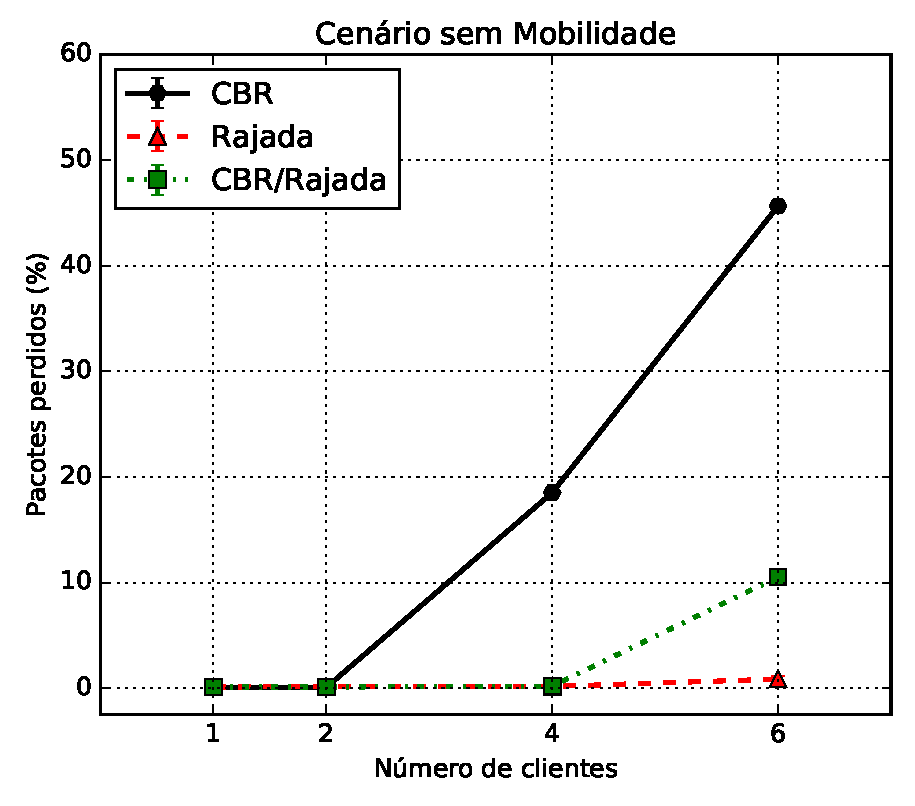
\includegraphics[width=0.48\textwidth]{img/perda_estatico_1_6_perc.eps}
	    \label{fig:perda_estatico_16_perc}
	}
	\subfigure[Porcentagem - Com mobilidade]{
		\includegraphics[width=0.48\textwidth]{img/perda_mobilidade_1_6_perc.eps}
	    \label{fig:perda_mobilidade_16_perc}
	}
	\caption{Resultados de perda de pacotes em porcentagem nos cenários sem e com mobilidade.}
	\label{fig:perda_perc}
\end{figure}

\subsection{Avaliação extra}

Para melhor visualização do impacto de utilização dos diferentes tipos de tráfegos com diferentes números de clientes, foi montado um conjunto de novas simulações com um número maior de clientes conectados ao AP. Assim, as configurações de comunicação são as mesmas utilizadas nas simulações anteriores, porém com o número de clientes variando em $6, 12, 24$ e $48$. A Tabela \ref{tab:parametros_extra} resume os parâmetros utilizados neste experimento extra.

\begin{table}[h]
\centering
\caption{Parâmetros de simulação para o com maior número de clientes}
\vspace{0.1cm} %espaco entre titulo e tabela
\label{tab:parametros_extra}
\begin{tabular}{ll}
\hline
 \textbf{Parâmetro} & \textbf{Valor} \\
\hline
 Tempo de simulação & 60 s \\
 Número de cliente & 6, 12, 24 e 48 \\
 Tamanho do cenário & 140m x 140m \\
 Padrão de comunicação & IEEE 802.11a \\
 Potência de transmissão & 16 dbm\\
 Velocidade dos clientes no cenário estático & 0 km/h\\
Velocidade dos clientes no cenário móvel & 3.6 a 7.2 km/h \\
 Modelo de mobilidade para nós estáticos & \texttt{ConstantPositionMobility} \\
 Modelo de mobilidade para nós móveis & \texttt{ConstantVelocityMobility} \\
 Taxa de dados & 512 kbps \\
 Tamanho do quadro UDP & 512 bytes\\
 Tamanho do quadro TCP & 1500 bytes \\
 Número de antenas no AP & 1 \\
 Aplicações & CBR, Rajada e CBR/Rajada\\
\hline
\end{tabular}
\end{table}

Desta forma, a Figura \ref{fig:atraso_extra} exibe o Atraso dos dois cenários, com 6, 12, 24 e 48 clientes atuantes na rede. Podemos observar que o atraso do tráfego em rajada fica superior ao CBR e CBR/Rajada a partir de 24 clientes tanto no cenário sem mobilidade quanto no cenário com mobilidade. Isso se justifica pelo elevado número de clientes e maior controle de tráfego realizado pelo TCP que é utilizado no tráfego em Rajada.

\begin{figure}[!ht]
	\centering
	\subfigure[Sem mobilidade]{
	    \includegraphics[width=0.48\textwidth]{img/delay_estatico_6_48.eps}
	    \label{fig:atraso_estatico_648}
	}
	\subfigure[Com mobilidade]{
		\includegraphics[width=0.48\textwidth]{img/delay_mobilidade_6_48.eps}
	    \label{fig:atraso_mobilidade_648}
	}
	\caption{Resultados de atraso nos cenários de 6, 12, 24 e 48 clientes sem e com mobilidade.}
	\label{fig:atraso_extra}
\end{figure}

A Figura \ref{fig:vazao_extra_648} exibe a Vazão para este mesmo cenário. Pode-se observar que a vazão mantém o comportamento de decaimento à medida que o número de clientes cresce na rede. O tráfego em Rajada mantém seu comportamento de menor vazão que os tráfegos CBR e CBR/Rajada. Um ponto importante para observação é que o padrão de menor vazão no cenário com mobilidade também se mantém aqui, reforçando ainda mais o que foi discutido acerca da mobilidade influenciar diretamente o comportamento da rede como um todo.

\begin{figure}[!ht]
	\centering
	\subfigure[Sem mobilidade]{
	    \includegraphics[width=0.48\textwidth]{img/vazao_estatico_6_48.eps}
	    \label{fig:vazao_estatico_648}
	}
	\subfigure[Com mobilidade]{
		\includegraphics[width=0.48\textwidth]{img/vazao_mobilidade_6_48.eps}
	    \label{fig:vazao_mobilidade_648}
	}
	\caption{Resultados de vazão nos cenários de 6, 12, 24 e 48 clientes sem e com mobilidade.}
	\label{fig:vazao_extra_648}
\end{figure}

A Figura \ref{fig:perda_extra} exibe os resultados de Perda de Pacotes em valores absolutos. Assim, podemos visualizar que o tráfego Rajada tem menores taxas de perda também nos cenários com maior número de clientes atuantes na rede. E ambos os tráfegos CBR e CBR/Rajada mantém seus comportamentos, onde o CBR/Rajada fica no meio termo entre CBR e Rajada por utilizar 50\% de cada tráfego. Aqui também podemos visualizar o impacto que a mobilidade exerce na rede.

\begin{figure}[!ht]
	\centering
	\subfigure[Sem mobilidade]{
	    \includegraphics[width=0.48\textwidth]{img/perda_estatico_6_48.eps}
	    \label{fig:perda_estatico_648}
	}
	\subfigure[Com mobilidade]{
		\includegraphics[width=0.48\textwidth]{img/perda_mobilidade_6_48.eps}
	    \label{fig:perda_mobilidade_648}
	}
	\caption{Resultados de perda de pacotes nos cenários de 6, 12, 24 e 48 clientes sem e com mobilidade.}
	\label{fig:perda_extra}
\end{figure}

Por fim, a Figura \ref{fig:perda_extra_perc} exibe as taxas de Perda de Pacotes em porcentagem para cada tráfego utilizado. Pode-se observar aqui que a mobilidade exerce influência significativa até no tráfego em Rajada, que utiliza o TCP e possui maior controle nas transmissões, fazendo com que a diferença de da taxa de perda suba de 4\% no cenário sem mobilidade para 20\% no cenário com mobilidade. Os outros tráfegos, conforme esperado, também sofrem aumentos em suas taxas de perda de pacotes.

\begin{figure}[!ht]
	\centering
	\subfigure[Porcentagem - Sem mobilidade]{
	    \includegraphics[width=0.48\textwidth]{img/perda_estatico_6_48_perc.eps}
	    \label{fig:perda_estatico_648_perc}
	}
	\subfigure[Porcentagem - Com mobilidade]{
		\includegraphics[width=0.48\textwidth]{img/perda_mobilidade_6_48_perc.eps}
	    \label{fig:perda_mobilidade_648_perc}
	}
	\caption{Resultados de perda de pacotes nos cenários de 6, 12, 24 e 48 clientes sem e com mobilidade.}
	\label{fig:perda_extra_perc}
\end{figure}


\section{Considerações finais}
\label{consideracoes}

Com base nos resultados apresentados na Seção \ref{resultados} pôde ser observado que os clientes que utilizam tráfego CBR para suas transmissões apresentaram maiores taxas de atraso comparados com os clientes que utilizam o tráfego em Rajada, tais taxas podem ser justificadas por conta do enchimento da fila de transmissão utilizada no protocolo UDP.

Em relação à Vazão, os clientes que utilizam CBR possuem maiores taxas de vazão em função do protocolo UDP não realizar nenhum controle na rede e tomar proveito de todo recurso que estiver disponível no momento da transmissão. Diferente do tráfego em Rajada, que faz uso do protocolo TCP, e existe um controle da rede para evitar colisões e, consequentemente, perda de pacotes.

No que se refere à Perda de Pacotes, observou-se que tanto o tráfego CBR quanto CBR/Rajada tiveram maiores taxas de perda de pacotes em comparação ao tráfego em Rajada. Isso de deu pelo fato do tráfego em Rajada utilizar o protocolo TCP e seus procedimentos de controle, diferente do UDP que não utiliza nenhum procedimento que garanta a entrega dos pacotes.

Observou-se também que em ambas avaliações com a presença de mobilidade nos clientes atuantes na rede as taxas de Atraso, Vazão e Perda de Pacotes sofreram impacto direto. Por fim, os resultados se mostram coerentes em ambos os cenários quando comparados Atraso, Vazão e Perda de Pacotes juntos. Onde, a medida que o número de clientes cresce na rede, a vazão diminui e, dependendo do tipo de tráfego, o atraso de entrega sofre aumenta ou diminui. 

\bibliographystyle{sbc}
\bibliography{sbc-template}

\newpage

%Codigofonte
\section*{Códigos utilizados nas simulações}
\label{codigofonte}

\subsection*{Código ``gerencia2018.cc" ~do NS3}

Foi utilizada a opção de passagem de parâmetros via terminal do simulador NS3, habilitada através da classe \texttt{ns3::CommandLine} (Linha 92). Assim, foram definidos os seguintes parâmetros para as simulações: \textit{seed, nwifi, mobilidade} e \textit{trafego}. Tais parâmetros são passados diretamente via terminal no \textit{script} \texttt{run\_gerencia2018.sh} que automatiza o processo de avaliação.

Para atribuir velocidade aos clientes no cenário com mobilidade foi utilizada a classe \texttt{ns3::ConstantVelocityMobility} e seu método para configuração de velocidade \texttt{SetVelocity}. Assim, a velocidade dos clientes foi atualizada a cada 0.5 segundos (Linha 46) no método \texttt{AtualizaVelocidade}. A velocidade configurada é definida a cada chamada de \texttt{AtualizaVelocidade} (Linha 200) obedecendo o intervalo definido entre 1 e 2 m/s, para que a velocidade de cada cliente seja ligeiramente diferente e deixe os experimentos mais próximo do que acontece no mundo real.

\begin{lstlisting}
/* Projeto: Rede 802.11 
 * Disciplina: MO655 - Gerencia de Redes de Computadores - 2018
 * Professor: Edmundo Madeira
 * Autores: Joahannes B. D. da Costa e Wellington V. Lobato Junior.
 * Email: joahannes, wellington{@lrc.ic.unicamp.br}
 * Laboratorio de Redes de Computadores - LRC
 */

#include "ns3/core-module.h"
#include "ns3/network-module.h"
#include "ns3/applications-module.h"
#include "ns3/wifi-module.h"
#include "ns3/mobility-module.h"
#include "ns3/internet-module.h"
#include "ns3/csma-module.h"
#include "ns3/point-to-point-module.h"
#include "ns3/netanim-module.h"
//Monitor de fluxo
#include "ns3/flow-monitor-module.h"
#include "ns3/flow-monitor.h"
#include "ns3/flow-monitor-helper.h"
#include "ns3/rng-seed-manager.h"
#include "ns3/random-variable-stream.h"

// Topologia da rede
//
//    10.1.1.0
// r0 *--------* AP
//               |        192.168.0.0
//               *    *    *    *    *    *   
//               |    |    |    |    |    |
//               c0   c1   c2   c3   c4   c5

using namespace ns3;

NS_LOG_COMPONENT_DEFINE ("projetoGerencia2018");

//Mobilidade para os dispositivos moveis
void AtualizaVelocidade(Ptr<Node> node) {
    Ptr<UniformRandomVariable> rvar = CreateObject<UniformRandomVariable>();
    Ptr <ConstantVelocityMobilityModel> mobility = node -> GetObject<ConstantVelocityMobilityModel>();
    
    double velocidade = rvar->GetValue(1, 2); // 3.6 a 7.2 km/h
    mobility->SetVelocity (Vector (velocidade, 0.0, 0.0));

    Simulator::Schedule (Seconds (0.5), AtualizaVelocidade, node);
}

void ImprimeMetricas (FlowMonitorHelper* fmhelper, Ptr<FlowMonitor> monitor, int trafego, int clientes){
	double totalThroughput = 0.0;
	monitor->CheckForLostPackets();
	std::map<FlowId, FlowMonitor::FlowStats> flowStats = monitor->GetFlowStats();
	Ptr<Ipv4FlowClassifier> classifier = DynamicCast<Ipv4FlowClassifier> (fmhelper->GetClassifier());

	for (std::map<FlowId, FlowMonitor::FlowStats>::const_iterator stats = flowStats.begin (); stats != flowStats.end (); ++stats)
	{
		Ipv4FlowClassifier::FiveTuple fiveTuple = classifier->FindFlow (stats->first);
		std::string flowidhost = "FlowID[" + std::to_string(stats->first) + "]";

		if(trafego == 0)
			std::cout << flowidhost <<"   Trafego   UDP" << std::endl;
		else if(trafego == 1)
			std::cout << flowidhost <<"   Trafego   TCP" << std::endl;
		else if(trafego == 2)
			std::cout << flowidhost <<"   Trafego   UDP/TCP" << std::endl;

		std::cout << flowidhost <<"   Clientes   " << clientes << std::endl; 
		std::cout << flowidhost <<"   Fluxo   "<< fiveTuple.sourceAddress <<" -----> "<<fiveTuple.destinationAddress<<std::endl;
		std::cout << flowidhost <<"   Duracao   " <<stats->second.timeLastRxPacket.GetSeconds() - stats->second.timeFirstTxPacket.GetSeconds()<<std::endl;
		totalThroughput = (stats->second.rxBytes * 8.0 / (stats->second.timeLastRxPacket.GetSeconds() - stats->second.timeFirstTxPacket.GetSeconds())/1024/1024);
		std::cout << flowidhost <<"   Vazao(Mbps)   "<< totalThroughput <<std::endl;
		std::cout << flowidhost <<"   Atraso   " << stats->second.delaySum.GetSeconds () / stats->second.rxPackets << std::endl;
		std::cout << flowidhost <<"   PacotesTransmitidos   " << stats->second.txPackets << std::endl;
		std::cout << flowidhost <<"   PacotesPerdidos   " << stats->second.lostPackets << std::endl;
	}
	Simulator::Schedule(Seconds(1),&ImprimeMetricas, fmhelper, monitor, trafego, clientes);
}


int main (int argc, char *argv[])
{
  uint16_t seed = 1; //Seeds
  bool verbose = true; //Verbose
  uint32_t nWifi = 1; //Quantidade de nos WiFi
  uint32_t apWifi = 1; //Quantidade de APs
  bool mobilidade = false; //Sem mobilidade por padrao
  double distance = 5.0; //Distancia entre os nos
  double simTime = 60.0; //Tempo de simulacao
  int trafego = 0; //UDP por padrao
  
//Parametros por linha de comando
  CommandLine cmd;
  cmd.AddValue ("seed", "Semente de simulacao", seed);
  cmd.AddValue ("nWifi", "Numero de clientes", nWifi);
  cmd.AddValue ("trafego", "(0) UDP, (1) TCP ou (2) para ambos", trafego);
  cmd.AddValue ("mobilidade", "(0) Sem mobilidade e (1) Com mobilidade", mobilidade);
  cmd.Parse (argc,argv);

//Seed
  RngSeedManager::SetSeed(12);
  RngSeedManager::SetRun(seed);
  Ptr<UniformRandomVariable> u = CreateObject<UniformRandomVariable> ();

  if (nWifi > 250)
  {
    std::cout << "Muitos nos wifi criados. Nosso limite e' 250." << std::endl;
    return 1;
  }

//Cria apenas nos WiFi
  NodeContainer wifiStaNodes;
  wifiStaNodes.Create (nWifi);

//Cria no AP
  NodeContainer wifiApNode;
  wifiApNode.Create (apWifi);

//Cria Router
  NodeContainer csmaNodes;
  csmaNodes.Add(wifiApNode.Get(0));
  csmaNodes.Create (1);

//Cria conexao entre Router e AP
  CsmaHelper csma;
  csma.SetChannelAttribute ("DataRate", StringValue ("100Mbps"));
  csma.SetChannelAttribute ("Delay", TimeValue (MilliSeconds (2)));

  NetDeviceContainer csmaDevices;
  csmaDevices = csma.Install (csmaNodes);

//Cria os nos WiFi e os interliga por meio de um canal
  YansWifiChannelHelper channel = YansWifiChannelHelper::Default ();
  YansWifiPhyHelper phy = YansWifiPhyHelper::Default ();
  phy.SetChannel (channel.Create ());

//Algoritmo de controle de de taxa, que neste caso e o AARF
  WifiHelper wifi;
  wifi.SetRemoteStationManager ("ns3::AarfWifiManager");

  WifiMacHelper mac;

//SSID do AP
  Ssid ssid = Ssid ("GerenciaRedes2018");
  //Clientes
  mac.SetType ("ns3::StaWifiMac", "Ssid", SsidValue (ssid), "ActiveProbing", BooleanValue (false));
  NetDeviceContainer staDevices = wifi.Install (phy, mac, wifiStaNodes);
  //AP
  mac.SetType ("ns3::ApWifiMac", "Ssid", SsidValue (ssid));
  NetDeviceContainer apDevices = wifi.Install (phy, mac, wifiApNode);

//Instancia a Mobilidade
  //AP_node
  Ptr<ListPositionAllocator> positionAlloc0 = CreateObject<ListPositionAllocator> ();
  positionAlloc0->Add (Vector(70, 70, 0));

  MobilityHelper mobilityAp;
  mobilityAp.SetMobilityModel("ns3::ConstantPositionMobilityModel");
  mobilityAp.SetPositionAllocator(positionAlloc0);
  mobilityAp.Install(wifiApNode);

  //Router
  Ptr<ListPositionAllocator> positionAllocRouter = CreateObject<ListPositionAllocator> ();
  positionAllocRouter->Add (Vector(0, 0, 0));

  MobilityHelper router;
  router.SetMobilityModel("ns3::ConstantPositionMobilityModel");
  router.SetPositionAllocator(positionAllocRouter);
  router.Install(csmaNodes.Get(1));

  //WiFi_nodes
  if (mobilidade == false)
  { 
    MobilityHelper mobilityWifi;
    mobilityWifi.SetPositionAllocator ("ns3::GridPositionAllocator",
        "MinX", DoubleValue (70.0),
        "MinY", DoubleValue (70.0),
        "DeltaX", DoubleValue (distance),
        "DeltaY", DoubleValue (distance),
        "GridWidth", UintegerValue (3),
        "LayoutType", StringValue ("RowFirst"));
    mobilityWifi.SetMobilityModel("ns3::ConstantVelocityMobilityModel");
    mobilityWifi.Install (wifiStaNodes);
  }
  else
  {
    MobilityHelper mobilityWifi;
    mobilityWifi.SetPositionAllocator("ns3::GridPositionAllocator",
        "MinX", DoubleValue (70.0),
        "MinY", DoubleValue (70.0),
        "DeltaX", DoubleValue (distance),
        "DeltaY", DoubleValue (distance),
        "GridWidth", UintegerValue (3),
        "LayoutType", StringValue ("RowFirst")); 
    mobilityWifi.SetMobilityModel("ns3::ConstantVelocityMobilityModel");
    mobilityWifi.Install (wifiStaNodes);

    //Atualiza velocidade dos nos
    for (uint16_t i = 0; i < nWifi; i++)
    {
      AtualizaVelocidade(wifiStaNodes.Get(i));
    }
  }

//Pilha de internet
  InternetStackHelper stack;
  stack.Install (csmaNodes);
  stack.Install (wifiStaNodes);

  Ipv4AddressHelper address;

  //Cria endereco para CSMA
  address.SetBase ("10.1.2.0", "255.255.255.0");
  Ipv4InterfaceContainer csmaInterfaces = address.Assign (csmaDevices);

  //Cria endereco para os Clientes
  address.SetBase ("192.168.0.0", "255.255.255.0");
  Ipv4InterfaceContainer interfacesAp = address.Assign (apDevices);
  Ipv4InterfaceContainer interfacesWifi = address.Assign (staDevices);

  if(trafego == 0)
  {
    //Aplicacao UDP
    uint16_t port = 9;
    for (uint32_t i = 0; i < wifiStaNodes.GetN(); i++)
    {
      uint16_t m_port = port + i;

      OnOffHelper onoff ("ns3::UdpSocketFactory", Address(InetSocketAddress(csmaInterfaces.GetAddress(1), m_port)));
      onoff.SetAttribute ("Remote",  AddressValue(InetSocketAddress(interfacesWifi.GetAddress(i), m_port)));
      onoff.SetAttribute ("OnTime", StringValue ("ns3::ConstantRandomVariable[Constant=1]"));
      onoff.SetAttribute ("OffTime", StringValue ("ns3::ConstantRandomVariable[Constant=0]"));
      onoff.SetAttribute ("DataRate", DataRateValue ( DataRate ("512kbps")));
      onoff.SetAttribute ("PacketSize", UintegerValue (478)); // +34 header

      ApplicationContainer server = onoff.Install(csmaNodes.Get(1));
      server.Start(Seconds (1.0));
      server.Stop(Seconds (simTime));

      PacketSinkHelper sink ("ns3::UdpSocketFactory", InetSocketAddress(interfacesWifi.GetAddress(i), m_port));

      ApplicationContainer client = sink.Install(wifiStaNodes.Get(i));
      client.Start(Seconds (2.0));
      client.Stop(Seconds (simTime));
    }
  }
  else if(trafego == 1)
  {
    //Aplicacao TCP
    uint16_t port = 8080;
    for (uint32_t i = 0; i < wifiStaNodes.GetN(); i++)
    {
      uint16_t m_port = port + i;

      OnOffHelper onoff ("ns3::TcpSocketFactory", Address(InetSocketAddress(csmaInterfaces.GetAddress(1), m_port)));
      onoff.SetAttribute ("Remote",  AddressValue(InetSocketAddress(interfacesWifi.GetAddress(i), m_port)));
      onoff.SetAttribute ("OnTime", StringValue("ns3::NormalRandomVariable[Mean=5.|Variance=1.|Bound=10.]"));
      onoff.SetAttribute ("OffTime", StringValue("ns3::NormalRandomVariable[Mean=7.|Variance=1.|Bound=10.]"));
      onoff.SetAttribute ("DataRate", DataRateValue ( DataRate ("512kbps")));
      onoff.SetAttribute ("PacketSize", UintegerValue (1440)); // +60 header

      ApplicationContainer server = onoff.Install(csmaNodes.Get(1));
      server.Start (Seconds (1.0));
      server.Stop (Seconds (simTime));

      PacketSinkHelper sink ("ns3::TcpSocketFactory", InetSocketAddress(interfacesWifi.GetAddress(i), m_port));

      ApplicationContainer client = sink.Install(wifiStaNodes.Get(i));
      client.Start(Seconds (2.0));
      client.Stop(Seconds (simTime));
      
    }

  }
  else if(trafego == 2)
  {
  	//Aplicacao UDP e TCP
  	for (uint32_t i = 0; i < wifiStaNodes.GetN(); i++)
  	{
  		uint32_t udp_port = 9;
  		uint32_t tcp_port = 8080;

  		if(i \% 2 == 0)
  		{
  			//Aplicacao UDP
			OnOffHelper onoff ("ns3::UdpSocketFactory", Address(InetSocketAddress(csmaInterfaces.GetAddress(1), udp_port+i)));
			onoff.SetAttribute ("Remote",  AddressValue(InetSocketAddress(interfacesWifi.GetAddress(i), udp_port+i)));
			onoff.SetAttribute ("OnTime", StringValue ("ns3::ConstantRandomVariable[Constant=1]"));
			onoff.SetAttribute ("OffTime", StringValue ("ns3::ConstantRandomVariable[Constant=0]"));
			onoff.SetAttribute ("DataRate", DataRateValue ( DataRate ("512kbps")));
			onoff.SetAttribute ("PacketSize", UintegerValue (478)); // +34 header

			ApplicationContainer server = onoff.Install(csmaNodes.Get(1));
			server.Start(Seconds (1.0));
			server.Stop(Seconds (simTime));

			PacketSinkHelper sink ("ns3::UdpSocketFactory", InetSocketAddress(interfacesWifi.GetAddress(i), udp_port+i));

			ApplicationContainer client = sink.Install(wifiStaNodes.Get(i));
			client.Start(Seconds (2.0));
			client.Stop(Seconds (simTime));
		}
  		else
  		{
			//Aplicacao TCP
			OnOffHelper onoff ("ns3::TcpSocketFactory", Address(InetSocketAddress(csmaInterfaces.GetAddress(1), tcp_port+i)));
			onoff.SetAttribute ("Remote",  AddressValue(InetSocketAddress(interfacesWifi.GetAddress(i), tcp_port+i)));
			onoff.SetAttribute ("OnTime", StringValue("ns3::NormalRandomVariable[Mean=5.|Variance=1.|Bound=10.]"));
			onoff.SetAttribute ("OffTime", StringValue("ns3::NormalRandomVariable[Mean=7.|Variance=1.|Bound=10.]"));
			onoff.SetAttribute ("DataRate", DataRateValue ( DataRate ("512kbps")));
			onoff.SetAttribute ("PacketSize", UintegerValue (1440)); // +60 header

			ApplicationContainer server = onoff.Install(csmaNodes.Get(1));
			server.Start (Seconds (1.0));
			server.Stop (Seconds (simTime));

			PacketSinkHelper sink ("ns3::TcpSocketFactory", InetSocketAddress(interfacesWifi.GetAddress(i), tcp_port+i));

			ApplicationContainer client = sink.Install(wifiStaNodes.Get(i));
			client.Start(Seconds (2.0));
			client.Stop(Seconds (simTime));
  		}
  	}
  }

  Ipv4GlobalRoutingHelper::PopulateRoutingTables ();

//Monitor de fluxo
  Ptr<FlowMonitor> monitor;
  FlowMonitorHelper fmhelper;
  monitor = fmhelper.InstallAll();

  Simulator::Stop (Seconds (simTime));
  Simulator::Run ();

//Imprime metricas n
  if (verbose)
  {
    ImprimeMetricas (&fmhelper, monitor, trafego, nWifi);
  }

  Simulator::Destroy ();
  return 0;
}
\end{lstlisting}

\subsection*{Script ``run\_gerencia2018.sh" ~para executar as simulações de forma automatizada}

Para execução dos diferentes tráfegos com as 33 \textit{seeds}, basta rodar o \textit{script} abaixo passando os devidos parâmetros, como por exemplo \texttt{./run\_gerencia.sh 33 6 0 0} que resulta em 33 simulações ($seed = 33$) no cenário com 6 clientes ($nWifi = 6$) utilizando tráfego CBR ($trafego = 0$) e sem mobilidade ($mobilidade = 0$).

Os parâmetros passados no \textit{script} são diretamente adicionados à chamada de simulação do NS3, da seguinte forma: \texttt{./waf --run "scratch/gerencia2018 --seed=\$i --nWifi=\$2 --trafego=\$3 --mobilidade=\$4"}. Onde \texttt{\$1} é o primeiro parâmetro passado, \texttt{\$2} o segundo parâmetro e assim sucessivamente.

\begin{lstlisting}
#!/bin/bash
#Autores: Joahannes B. D. da Costa e Wellington V. Lobato Junior
#Data: 23.09.2018
#Nota: script para rodar simulacao de MO655 - Gerencia de Redes - 2018
#Rodar: ./run_gerencia.sh numero_seeds numero_clientes trafego mobilidade

seeds=$1
#$2 = clientes
#$3 = trafego

#Vai para diretorio ns-3.29
cd ..

echo
echo " * MO655 - Gerencia de Redes - 2018"
echo " * Numero de seeds: $1"
echo " * Numero de clientes: $2"
if [ $4 == 0 ]
then
	echo " * Mobilidade: Ausente"
else
	echo " * Mobilidade: Presente"
fi
if [ $3 == 0 ]
then
	echo " * Trafego: UDP"
elif [ $3 == 1 ]
then
	echo " * Trafego: TCP"
else
	echo " * Trafego: 50% UDP e 50%TCP"
fi

for ((i=0; i<$seeds; i++))
do
	if [ $4 == 0 ]
	then
		#Controle para mensagens
		if [ $3 == 0 ]
		then
			echo "Executando seed [$i] com $2 clientes ESTATICOS e trafego UDP..."
			#Chamada da simulacao
			./waf --run "scratch/gerencia2018 --seed=$i --nWifi=$2 --trafego=$3 --mobilidade=$4" > resultados/UDP/results-$2-est-UDP-$i.txt 2>&1
		elif [ $3 == 1 ]
		then
			echo "Executando seed [$i] com $2 clientes ESTATICOS e trafego TCP..."
			#Chamada da simulacao
			./waf --run "scratch/gerencia2018 --seed=$i --nWifi=$2 --trafego=$3 --mobilidade=$4" > resultados/TCP/results-$2-est-TCP-$i.txt 2>&1
		else
			echo "Executando seed [$i] com $2 clientes ESTATICOS e trafegos UDP/TCP..."
			#Chamada da simulacao
			./waf --run "scratch/gerencia2018 --seed=$i --nWifi=$2 --trafego=$3 --mobilidade=$4" > resultados/UDP-TCP/results-$2-est-AMBOS-$i.txt 2>&1
		fi
	else
		#Controle para mensagens
		if [ $3 == 0 ]
		then
			echo "Executando seed [$i] com $2 clientes MOVEIS e trafego UDP..."
			#Chamada da simulacao
			./waf --run "scratch/gerencia2018 --seed=$i --nWifi=$2 --trafego=$3 --mobilidade=$4" > resultados/UDP/results-$2-mov-UDP-$i.txt 2>&1
		elif [ $3 == 1 ]
		then
			echo "Executando seed [$i] com $2 clientes MOVEIS e trafego TCP..."
			#Chamada da simulacao
			./waf --run "scratch/gerencia2018 --seed=$i --nWifi=$2 --trafego=$3 --mobilidade=$4" > resultados/TCP/results-$2-mov-TCP-$i.txt 2>&1
		else
			echo "Executando seed [$i] com $2 clientes MOVEIS e trafegos UDP/TCP..."
			#Chamada da simulacao
			./waf --run "scratch/gerencia2018 --seed=$i --nWifi=$2 --trafego=$3 --mobilidade=$4" > resultados/UDP-TCP/results-$2-mov-AMBOS-$i.txt 2>&1
		fi
	fi
done

echo "----------------------------------------------------"

#EOF
\end{lstlisting}

\end{document}
